\documentclass[titlepage,table]{article}

% Sprach-Pakete:
\usepackage[ngerman]{babel}     % Deutsche Silbentrennung, Begriffe & Typografie
\usepackage[T1]{fontenc}        % Korrekte Darstellung & Trennung von Umlauten

% Layout-Einstellungen
\frenchspacing                  % Einheitlicher Abstand nach Satzzeichen (keine extra Leerzeichen)
\tolerance=9000                 % Erlaubt größere Lücken zwischen Wörtern, um unschöne Umbrüche zu vermeiden
\usepackage{parskip}            % Entfernt Absatzeinrückung und fügt Abstand zwischen Absätzen hinzu
\usepackage{lmodern}            % Schriftart Latin Modern
\usepackage{titlesec}           % Benutzerdefinierte Überschriften
\usepackage{lastpage}           % Gesamtseitenzahl abrufen
\usepackage{fancyhdr}           % Für individuelle Kopf- und Fußzeilen -> s.u.
\usepackage{geometry}           % Ermöglicht benutzerdefinierte Seitenränder
\geometry{a4paper, left=25mm, right=25mm, top=3.5cm, bottom=2.5cm} % Ränder setzen

% praktische Pakete
\usepackage{hyperref}           % Aktiviert klickbare Links (URLs, Querverweise, Inhaltsverzeichnis)
\usepackage{color}              % Ermöglicht farbige Darstellung von Text und Elementen
\usepackage{comment}            % große Textblöcke auskommentieren -> \begin{comment} ... \end{comment}
\usepackage{siunitx}            % Einheiten -> \SI{wert}{\einheit}

% Bilder / PDFs
\usepackage{graphicx}           % Fügt Bilder (JPG, PNG, PDF) in LaTeX-Dokumente ein    -> \includegraphics[width=...]{bild.png}
\usepackage[inkscapeformat=png]{svg} % Ermöglicht SVG-Grafiken, konvertiert zu PNG
\usepackage{subcaption}         % Ermöglicht mehrere Teilabbildungen mit Untertiteln
\usepackage{pdfpages}           % Einfügen von PDF-Dokumenten -> \includepdf[pages={...}]{dokument.pdf}

% Tabellen
\usepackage{hhline}             % Erlaubt doppelte und selektive Linien in Tabellen
\usepackage{multirow}           % Erlaubt das Zusammenfassen mehrerer Zeilen in Tabellen
\usepackage[table]{xcolor}      % Ermöglicht das Färben von Tabellenzellen -> \cellcolor{color}
\usepackage{booktabs}           % Schönere Tabellenlinien -> \toprule, \midrule, \bottomrule

% Quellcode
\usepackage{listings, pmboxdraw} % Quellcode einbinden und optisch ansprechend rahmen

% Mathematik
\usepackage{amsmath}            % Mathematische Symbole, align-Umgebung (&=)
\usepackage{amssymb}            % Extra Mathe-Symbole (z. B. Mengen, Relationen)
\usepackage[makeroom]{cancel}   % Streicht mathematische Ausdrücke durch (mit zusätzlichem Raum)

% Literaturverzeichnis
\usepackage[backend=bibtex, sorting=nyt, urldate=long]{biblatex} % BibTeX-Backend, sortiert nach Name, Jahr, Titel; langes URL-Abrufdatum

% Abkürzungsliste
\usepackage{acronym} % -> \ac{...} 

% Anhänge
\usepackage[toc,page]{appendix} % Ermöglicht Anhänge mit eigener Überschrift


%---------------------------------------------------------------------------------------

\begin{document}
% 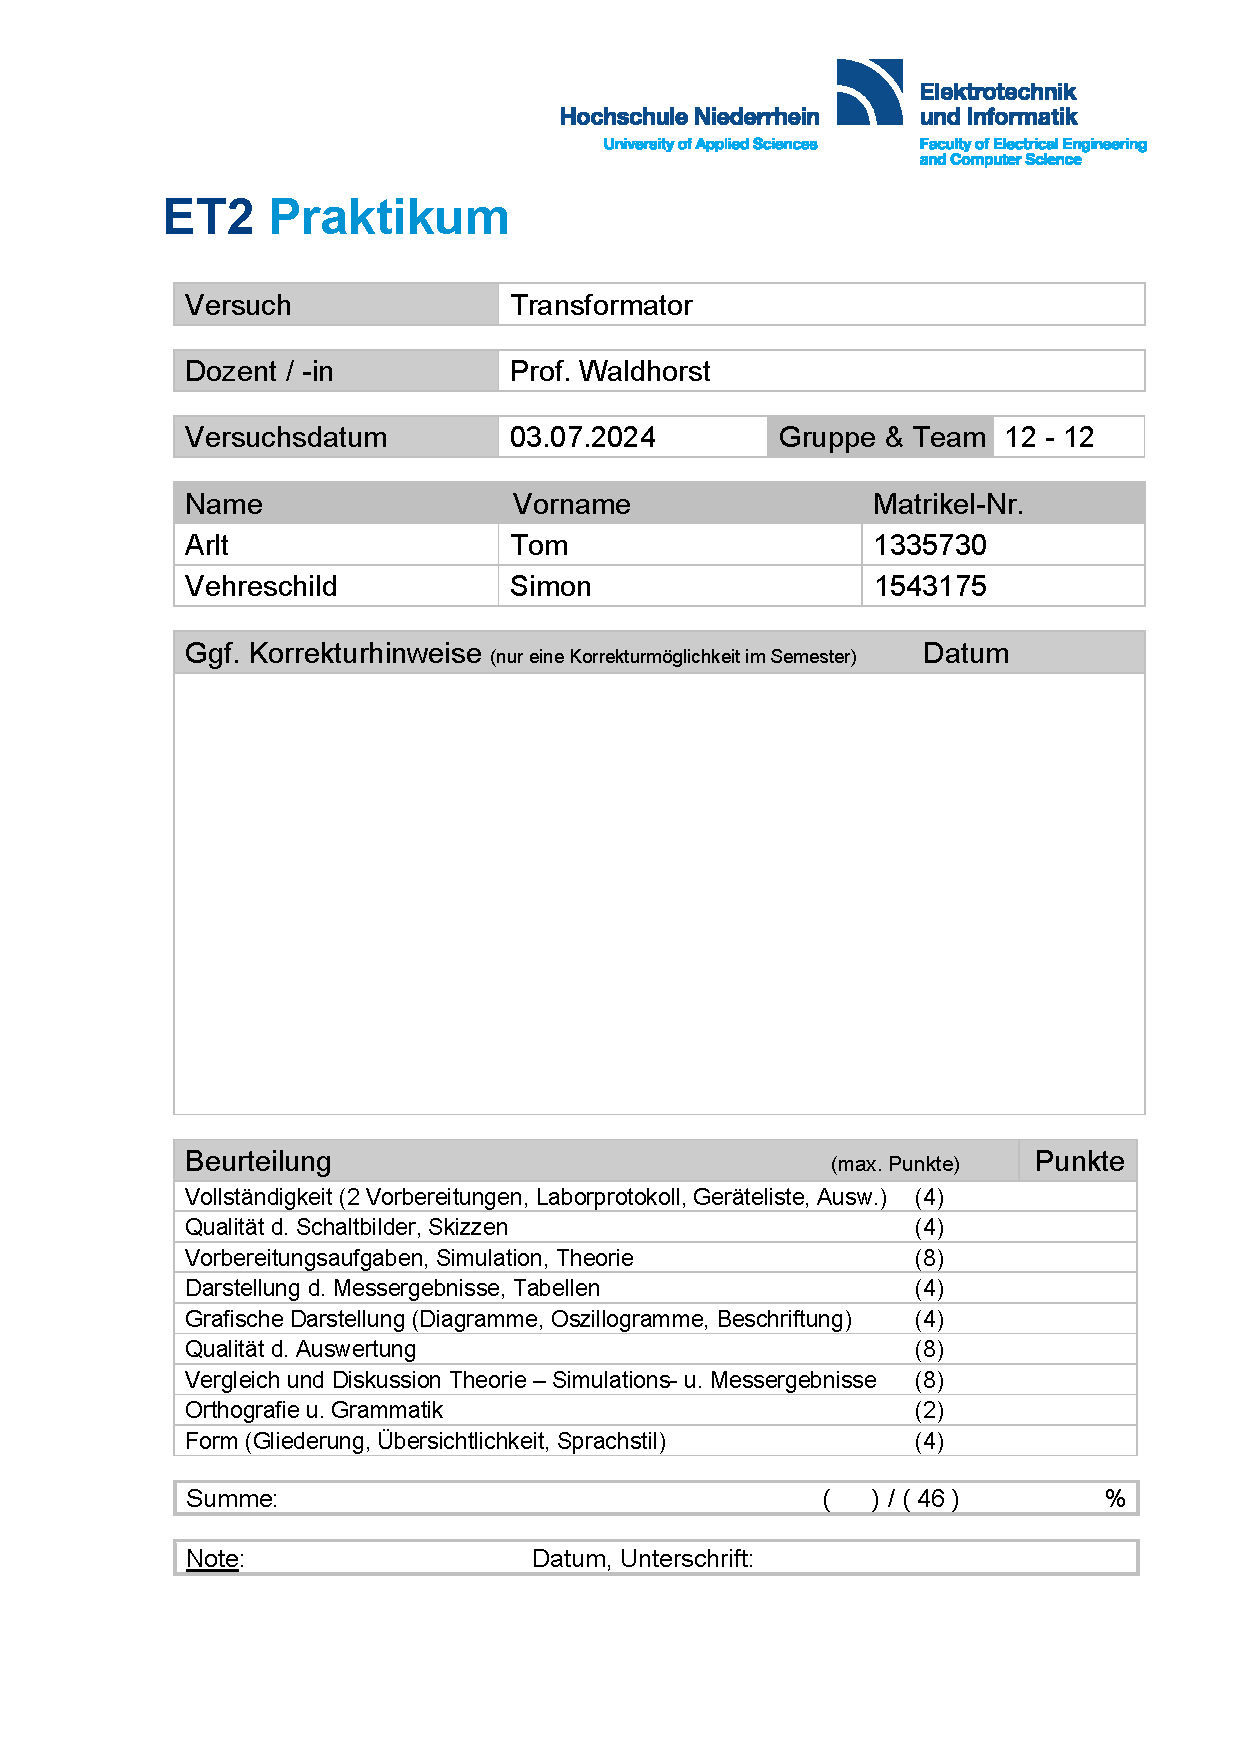
\includepdf{chapters/Deckblatt.pdf}                               ?????
% \input{chapters/titlepage}                                        ?????

% Kopf- und Fußzeilen
\pagestyle{fancy}                                    % Aktiviert individuelle Kopf- und Fußzeilen
\fancyfoot{}                                         % Löscht alle Standard-Fußzeilen
\fancyfoot[C]{Seite \thepage~von~\pageref{LastPage}} % Fußzeile mit "Seite X von Y"     % Praktisch auch:[RO,LE]
\fancyfoot[R]{Simon Vehreschild}                     % Rechte Seite: Autorname
\fancyfoot[L]{Latex Anleitung}                       % Linke Seite: Dokumentname#
\renewcommand{\footrulewidth}{0.4pt}                 % Linie über der Fußzeile
\fancyhead{}                                         % Löscht alle Standard-Kopfzeilen
\renewcommand{\headrulewidth}{0.4pt}
\fancyhead[R]{\leftmark}                             % Kopfzeile: Kapitelname
\fancyhead[L]{\includegraphics[width=2cm]{logo.png}} % Logo links in der Kopfzeile

\tableofcontents
\newpage


% \renewcommand{\labelenumi}{\alph{enumi}}
%\pagenumbering{arabic} %%ggf \fancyfoot[C]{Seite \thepage~von~\pageref{LastPage}}   \usepackage{lastpage}

% \renewcommand{\familydefault}{\sfdefault}


% Text

\input{Kapitel/Übersicht.tex}

\end{document}